\documentclass[varwidth=40cm]{standalone}
\usepackage{tikz}
\usepackage{style}

\begin{document}
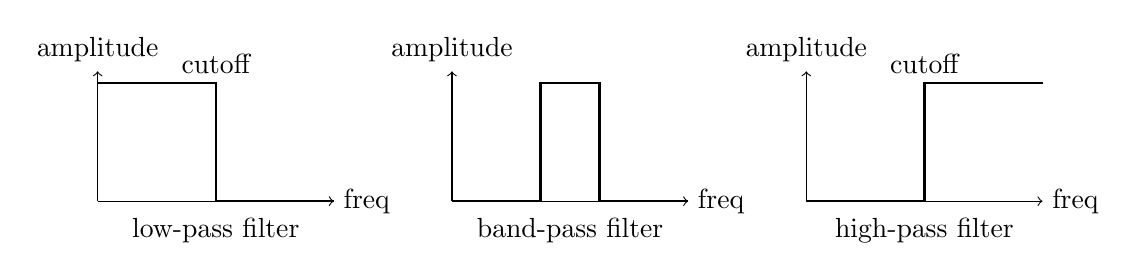
\begin{tikzpicture}[scale=1.5]
  \draw[->] (0,0) -- (2,0) node[right] {freq};
  \draw[->] (0,0) -- (0,1.1) node[above] {amplitude};
  \draw[thick] (0,1) -- (1,1) -- (1,0) -- (2,0);
  \draw (1,1) node[above] {cutoff};
  \draw (1,-.25) node {low-pass filter};

  \begin{scope}[shift={(3,0)}]
    \draw[->] (0,0) -- (2,0) node[right] {freq};
    \draw[->] (0,0) -- (0,1.1) node[above] {amplitude};
    \draw[thick] (0,0) -- (.75,0) -- (.75,1) -- (1.25,1) -- (1.25,0) -- (2,0);
    \draw (1,-.25) node {band-pass filter};
  \end{scope}

  \begin{scope}[shift={(6,0)}]
    \draw[->] (0,0) -- (2,0) node[right] {freq};
    \draw[->] (0,0) -- (0,1.1) node[above] {amplitude};
    \draw[thick] (0,0) -- (1,0) -- (1,1) -- (2,1);
    \draw (1,1) node[above] {cutoff};
    \draw (1,-.25) node {high-pass filter};
  \end{scope}
\end{tikzpicture}
\end{document}
